\section{Reducing the MPI grid setup and initial load balancing overhead}


\chapterDescription
  {
    Around 30 minutes.
  }
  {
    A working MPI code.
  }


In this section, we assume that you've a reasonable load balancing and that you
were able to postprocess your performance analysis outputs. We discuss issues
that arise over and over again for parallel applications.


\subsection{Massive grid on rank 0 with long redistribution phase
afterwards}

\begin{center}
  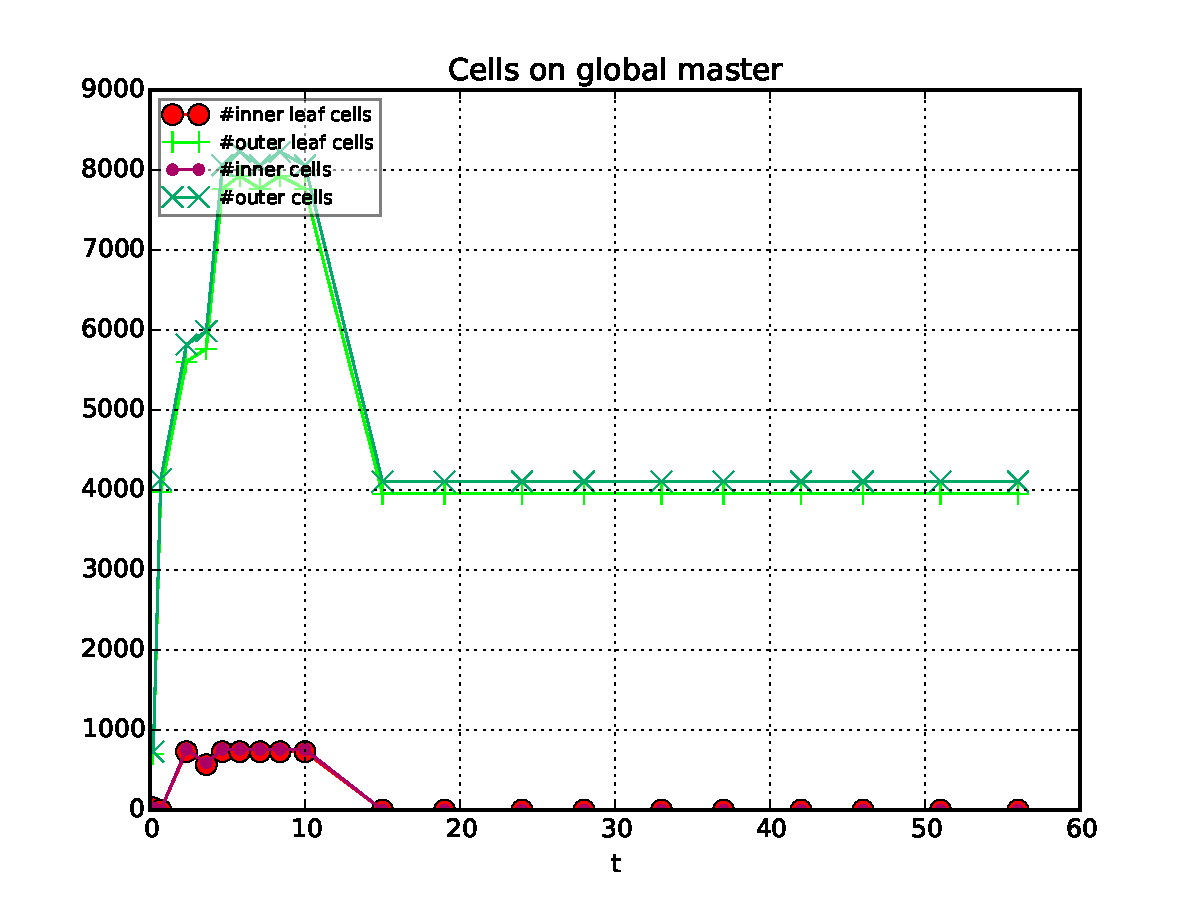
\includegraphics[width=0.5\textwidth]{61_mpi-setup/performance-analysis-output.pdf}
\end{center}


\begin{smell}
There are ranks (notably rank 0) that are assigned lots of cells and vertices
and then this number decreases though the grid should be more or less static.
\end{smell}

\noindent
We observe this behaviour either through a performance analysis (see plot above)
or by outputs from the state where the grid depth immediately goes up to the
maximum depth while the load balancing still splits up things. 
The iterations already are very expensive; obviously as the grid is already in
place but the ranks are not all employed.


The reason for this behaviour can be found in the semantics of
\texttt{createVertex} and \linebreak
\texttt{touchVertexFirstTime}.
Both operations try to refine the grid around the respective vertex immediately. 
Only if circumstances such as a parallel partitioning running through this
vertex---the refinement instruction then first has be distributed to all ranks
holding a copy of this vertex---do not allow Peano to realise the refinement
immediately, the refinement is postponed to the next iteration.
In many parallel codes, all the refinement calls pass through immediately on
rank 0 before it can spawn any rank.
This leads to the situation that the whole grid is in one sweep built up on the
global master and afterwards successively distributed among the ranks.


Such a behaviour is problematic: the global rank might run out of memory, lots
of data is transferred, and the sweeps over the whole grid on rank 0 are
typically pretty expensive. 
A distributed grid setup is advantageous.

\begin{solution}
Switch from an aggressive
refinement into an iterative grid refinement strategy to allow the ranks to
deploy work throughout the grid construction and thus build up the grid in parallel and avoid the transfer of whole grid
blocks due to rebalancing.
\end{solution}

\noindent
The simplest materialisation of this idea is to 
move your \texttt{refine()} calls from the creational or touch first
events into \texttt{touchVertexLastTime()}:
As a consequence, setting up a (rather regular) grid of depth $k$ requires at
least $k$ iterations.

\begin{remark}
 I typically extract the intial grid construction decision into a function of 
 its own. If \texttt{-DParallel} is used, I invoke grid constructions only 
 from \texttt{touchVertexLastTime}. Otherwise, I use it in the creational 
 routines for inner and boundary vertices. For this strategy, we have to ensure
 that touch last is not set to \texttt{Nop} in the specification attributes if
 we compile with MPI.
\end{remark}

In a second step, you might consider to extend your grid only every second
traversal.
Everytime you rebalance your grid, Peano disables dynamic load balancing
for a couple of iterations (three or four). Throughout these iterations, it
can recover all adjacency information if the grid itself changes as well.
Consequently, it does make sense to add a couple of adapter runs after each
grid modification that to not change the grid structure: When you know that
you have an adapter that changes the grid, apply afterwards an adapter that
does not change the grid for a couple of times. This way, you ensure that no
mpi rank runs out of memory. The grid generation does not overtake the rebalancing.
I often do not use an additional adapter but ensure that refines are only called
if the tree traversal direction is not inverted: 
Peano runs forth and back through the grid, so this effectively switches off
refinement every second iteration. 

The deluxe version is a code that refines only if the previous grid traversal
did not change the mesh, if no load balancing is going anymore and, for example,
\texttt{isTraversalInverted()} does not hold. This postpones any refinement
further.
However, such an approach is a bad idea if no idle nodes are available anymore. 
In this case, it is better not to veto the refinement anymore.
This situation is discussed in the following bad smell, where we propose a
sophisticated solution to both smells.



\subsection{Incremental, slow grid setup though detailed grid structure is
known/all nodes are already busy}


\begin{smell}
The grid is static, but, nevertheless, Peano needs lots of iterations to finally
build it up. Even worse, there are no idle nodes left and we know analytically
what the grid should look like.
The grid construction thus should rush through in one iteration.
\end{smell}


\noindent
Peano exchanges the vertices along a domain boundary after each traversal.
At the same time, it tries to refine a vertex with a refinement flag as soon as
possible: 
if a code sets a refine command upon creation of a vertex or when a vertex is
loaded for the very first time, it immediately refined.
If refine is called later throughout the traversal, Peano has to memorise the 
refinement request and wait for the subsequent traversal as all adjacent cells
have to anticipate an ongoing refinement but some have already been processed.
To ensure that the grid is always consistent, vertices at a domain boundary
never can be refined immediately. 
These guys are exchanged after each traversal and merged with their counterpart
on other ranks prior to the next usage. 
Refinement triggers thus never are available immediately on other ranks---these
vertices are replicated not held synchronous.

This behaviour implies that the grid can be built up at most by one level per
iteration along domain boundaries.
Therefore, we often see codes running many iterations until a regular grid is
built up completely.
Often, this is not necessary as all ranks would know without any data
exchange where to refine (a certain mesh size might be prescribed, e.g.).
For this case, Peano provides a function \texttt{enforceRefine} in the parallel
mode that tells the code not to bother about data consistency and to refine 
everywhere. 
Basically, the user tells the grid that he accepts responsibility to call 
\texttt{enforceRefine} on all replicants of a vertex.

We have to be very careful to use the enforced refinement.
We may use it if and only if there are no more idle nodes available and if all
previous forks and joins have successfully passed through. 
This is furthermore information that is available only on the global master. 

We thus propose to augment the \texttt{State.def} by a new flag:
\begin{code}
  #ifdef Parallel
  enum GridConstructionState {
    Default, Veto, Aggressive
  };
  
  parallelise persistent GridConstructionState  gridConstructionState; 
  #endif
\end{code}

\noindent
Per rank, we now create a copy of the global state that is propagated through
the tree (the state is used to determine the refinement strategy)
\begin{code}
  _localState = solverState;
\end{code}

\noindent
and we furthermore plug into the mapping's \texttt{endIteration} on modify this
global state on the global master. 
It has to be the global master as only the global master may ask the node pool
about idle nodes. 
Furthermore, it knows the (fork/join) state of all other ranks.
It is important to plug into \texttt{endIteration}, as this is the earliest
point where we have all information about the grid state at hands. 
The underlying status variables all are accumulated, i.e.~they might be already
cleared in the subsequent \texttt{beginIteration}:
\begin{code}
  if ( tarch::parallel::Node::getInstance().isGlobalMaster() ) {
    solverState.updateRegularInitialGridRefinementStrategy();
  }
\end{code}

\noindent
The state transitions then are
\begin{code}
void exahype::State::updateRegularInitialGridRefinementStrategy() {
  assertion( tarch::parallel::Node::getInstance().isGlobalMaster() );

  #ifdef Parallel
  if (
    tarch::parallel::Node::getInstance().getNumberOfNodes()==1
    ||
    _stateData.getGridConstructionState()==exahype::records::State::Aggressive
  ) {
    _stateData.setGridConstructionState( exahype::records::State::Aggressive );
  }
  else if (
    tarch::parallel::NodePool::getInstance().getNumberOfIdleNodes()==0
    &&
    isGridStationary()
  ) {
    _stateData.setGridConstructionState( exahype::records::State::Aggressive );
  }
  else if (
    isInvolvedInJoinOrFork()
    ||
    !isTraversalInverted()
    ||
    !isGridStationary()
  ) {
    _stateData.setGridConstructionState( exahype::records::State::Veto );
  }
  else {
    _stateData.setGridConstructionState( exahype::records::State::Default );
  }
  #endif
}

bool myproject::State::refineInitialGridInCreationalEvents() const {
  #ifdef Parallel
  return _stateData.getGridConstructionState() == myproject::records::State::Aggressive;
  #else
  return true;
  #endif
}

bool myproject::State::refineInitialGridInTouchVertexLastTime() const {
  #ifdef Parallel
  return _stateData.getGridConstructionState() != myproject::records::State::Veto;
  #else
  return false;
  #endif
}
\end{code}

\noindent
and we invoke our refinement from the creational vertex events as well as
\texttt{touchVertexLastTime} if the corresponding state predicates hold.
Finally, we make the refinement fall back to an enforced refinement if the state
permits us to do so:
\begin{code}
void myproject::mappings::RegularMesh::refineVertexIfNecessary(
  exahype::Vertex&                              fineGridVertex,
  const tarch::la::Vector<DIMENSIONS, double>&  fineGridH,
  bool                                          isCalledByCreationalEvent
) const {
  if (
    fineGridVertex.getRefinementControl() == Vertex::Records::Unrefined
    &&
    I want to refine and know this a priori
  ) {
    #ifdef Parallel
    if (isCalledByCreationalEvent) {
      fineGridVertex.enforceRefine();
    }
    else {
      fineGridVertex.refine();
    }
    #else
    fineGridVertex.refine();
    #endif
  }
}
\end{code}






\subsection{The load balancing kicks in immediately while I build up my grid but it
yields non-reasonable partitions}


\begin{smell}
The code runs over the grid a couple of times and starts to distribute the
domain level-by-level as we rely on an incremental build-up. This is however not
clever as it turns out later throughout the grid construction that some regions
are heavily refined while others remain coarse.
\end{smell}


\noindent
If this is the case, it might be reasonable to build up the grid up to a certain
level where grid characteristics become visible, and to switch off the load
balancing while you do so.
Afterwards, load balancing can be enabled and should yield better results. 
Peano allows you to switch off the load balancing, but you have to do this on
each individual rank. 

\begin{code}
peano::parallel::loadbalancing::Oracle::getInstance().activateLoadBalancing(false);
\end{code}


You might want to use
\begin{code}
void myproject::runners::Runner::runGlobalStep() {
  // assertion( !peano::parallel::loadbalancing::Oracle::getInstance().
  // isLoadBalancingActivated() );

  peano::parallel::loadbalancing::Oracle::getInstance().activateLoadBalancing(false);
}
\end{code}

\noindent
to switch off load balancing globally.


